\documentclass[10pt]{article}
\oddsidemargin = 0.2in
\topmargin = -0.5in
\textwidth 6in
\textheight 8.5in

\usepackage{graphicx,bm,amssymb,amsmath,amsthm} % Figures and maths
\usepackage[colorlinks]{hyperref} % Hyperlinks
\usepackage[capitalise, nameinlink]{cleveref} % Better referencing
\usepackage{array}
\usepackage{showlabels} % Shows eq, fig, etc labels
\usepackage{siunitx} % SI units

% -------------------------------------- macros --------------------------
% general ...
\newcommand{\bi}{\begin{itemize}}
\newcommand{\ei}{\end{itemize}}
\newcommand{\ben}{\begin{enumerate}}
\newcommand{\een}{\end{enumerate}}
\newcommand{\be}{\begin{equation}}
\newcommand{\ee}{\end{equation}}
\newcommand{\bea}{\begin{eqnarray}} 
\newcommand{\eea}{\end{eqnarray}}
\newcommand{\ba}{\begin{align}} 
\newcommand{\ea}{\end{align}}
\newcommand{\bse}{\begin{subequations}} 
\newcommand{\ese}{\end{subequations}}
\newcommand{\bc}{\begin{center}}
\newcommand{\ec}{\end{center}}
\newcommand{\bfi}{\begin{figure}}
\newcommand{\efi}{\end{figure}}
\newcommand{\ca}[2]{\caption{#1 \label{#2}}}
\newcommand{\ig}[2]{\includegraphics[#1]{#2}}
\newcommand{\bmp}[1]{\begin{minipage}{#1}}
\newcommand{\emp}{\end{minipage}}
\newcommand{\pig}[2]{\bmp{#1}\includegraphics[width=#1]{#2}\emp} % mp-fig, nogap
\newcommand{\bp}{\begin{proof}}
\newcommand{\ep}{\end{proof}}
\newcommand{\ie}{{\it i.e.\ }}
\newcommand{\eg}{{\it e.g.\ }}
\newcommand{\etal}{{\it et al.\ }}
\newcommand{\etc}{{\it etc.\ }}
\newcommand{\pd}[2]{\frac{\partial #1}{\partial #2}}
\newcommand{\pdc}[3]{\left. \frac{\partial #1}{\partial #2}\right|_{#3}}
\newcommand{\infint}{\int_{-\infty}^{\infty} \!\!}      % infinite integral
\newcommand{\tbox}[1]{{\mbox{\tiny #1}}}
\newcommand{\mbf}[1]{{\mathbf #1}}
\newcommand{\half}{\mbox{\small $\frac{1}{2}$}}
\newcommand{\C}{\mathbb{C}}
\newcommand{\N}{\mathbb{N}}
\newcommand{\R}{\mathbb{R}}
\newcommand{\Z}{\mathbb{Z}}
\newcommand{\RR}{\mathbb{R}^2}
\renewcommand{\d}{\mathrm{d}} % Upright differential
\newcommand{\ve}[4]{\left[\begin{array}{r}#1\\#2\\#3\\#4\end{array}\right]}  % 4-col-vec
\newcommand{\vt}[2]{\left[\begin{array}{r}#1\\#2\end{array}\right]} % 2-col-vec
\newcommand{\bigO}{{\mathcal O}}
\newcommand{\qqquad}{\qquad\qquad}
\newcommand{\qqqquad}{\qqquad\qqquad}
\newcommand{\eps}{\epsilon}
\DeclareMathOperator{\Span}{Span}
\DeclareMathOperator{\im}{Im}
\DeclareMathOperator{\re}{Re}
\DeclareMathOperator{\vol}{vol}
\newtheorem{thm}{Theorem}
\newtheorem{cnj}[thm]{Conjecture}
\newtheorem{lem}[thm]{Lemma}
\newtheorem{cor}[thm]{Corollary}
\newtheorem{pro}[thm]{Proposition}
\newtheorem{rmk}[thm]{Remark}
% this work...
\newcommand{\om}{\omega}
\newcommand{\g}{\gamma}
\newcommand{\te}{\tilde\eta}
\crefalias{prop}{Proposition}
% Review
\newcommand{\Alex}[1]{{\color{orange}#1}}
\newcommand{\Fruzsi}[1]{{\color{blue}#1}}

\begin{document}

\title{Analysis of an iteration for non-oscillatory solutions to the Riccati form of the phase function for 2nd-order linear ODEs}

\author{Fruzsina J.\ Agocs and Alex H.\ Barnett}
\date{\today}
\maketitle

\begin{abstract}
We gather basic definitions and error analysis.
\end{abstract}

\section{Introduction}

The efficient numerical solution of highly oscillatory ordinary differential
equations (ODEs) has long been a challenge and focus of computational
mathematics. A wide range of specialised methods exists for dealing with ODEs
with different structures, thorough reviews of which are found in
\cite{petzold1997,engquist2009}. Due to the large number of ways oscillations
in ODEs can arise, only a handful of methods have been designed to deal with any
given type of oscillatory ODE.  

In this work we focus on ODEs of a particular form: the general, linear, second
order ODE for a single variable, or the generalised single harmonic oscillator.
Since approximation by harmonic oscillators is ubiquitous in physical models,
this ODE, albeit simple-looking, is pivotal in many computational physics problems.

The ODE of interest takes the form
%We are interested in efficient numerical solution of
%the oscillatory linear 2nd-order ordinary differential equation (ODE)
\be
u''(t) + 2\g(t) u'(t) + \om^2(t)u(t) = 0, \qquad t \in (t_0,t_1).
\label{ode}
\ee
We choose to solve the ODE as an initial value problem (IVP) by specifying the initial conditions
\begin{align} % \ba, \ea doesn't work here, LaTeX complains
    u(t_0) &= u_0 \label{ic0} \\
    u'(t_0) &= u'_0. \label{ic1}
\end{align}
%Here the local frequency function $\om(t)$ is purely real or purely imaginary.
In regions where $\om \gg 1$, the solution $u$ is oscillatory, meaning that on some local
scale it is approximately $a e^{i\om_0t} + b e^{-i\om_0t}$ where $\om_0$ is the local value of $\om(t)$.
Conventional ODE integrators then require discretization with several
time-points per local period $2\pi/\om$, which can be prohibitively slow.
This has led to the development of more efficient solvers for this
high-frequency case. However, as we will review later, none of these methods so
far have been robust or general enough to solve the general ODE to arbitrary
accuracy in both the highly oscillatory and the slowly-varying regime.   

In this work we only consider regions where $\om(t)$ and $\g(t)$ are real-valued and $\om(t)$ is positive, but 
one may also consider $q(t):=\om^2(t)$ real and allow evanescent
$q<0$ regions, where the solution $u$ has rapid growth and decay.
%For now we ignore the real-valued damping function $\g(t)$,
%setting $\g \equiv =0$. *** to include.

% Asymptotic methods: WKB, oscode, QML
% Not asymptotics: Bremer
A large class of efficient numerical solvers for highly oscillatory ODEs of the above form makes use of asymptotic expansions. 


WKB blah.
QML.
oscode.
Recently Bremer following Bremer--Rokhlin has proposed an efficient
method
which requires $\bigO(1)$ effort per $t$ evaluation for such an
oscillatory solution, by solving for a nonoscillatory
phase function for Kummer's equation.
The existence of such a nonoscillatory phase function
(meaning that its Fourier transform is exponentially small in $\om$ ***
look up) is proven by Bremer--Rokhlin.
Despite this, finding initial conditions on the phase function leading to
a nonoscillatory solution is challenging.
Those authors proposed a
``windowing'' method to numerically find such a global phase function
on an interval:
the idea is to use a $C^\infty$ partition of unity near the upper end of the interval ($t=1$) to smoothly ``blend'' $q$ to
a constant function, then integrate backwards from the constant region
down to the lower end ($t=0$)
finally integrating $t\in[0,1]$ forward using the original $q$.
This exploits the facts that i) a nonoscillatory phase function for
the constant case $q(t) = \om_0^2$ is simple to write down, and
ii) the smooth window allows
the nonlinear Kummer oscillator to make a smooth (in physics
terminology ``adiabatic'') transition which excites
only exponentially small oscillation amplitude.
ETC.

Here we present an alternative approach using
an asymptotic expansion for a nonoscillatory
Riccati phase function, meaning simply that the
phase function is the logarithmic derivative $x(t) = (\log u(t))'$.
Our expansion is simpler than the traditional WKB expansion,
although of similar accuracy.
One novelty is that we
implement the expansion iteratively
using high-order numerical differentiation, rather
than algebraically (as WKB is usually applied).
The iteration does not introduce oscillatory contributions,
hence finds a nonoscillatory approximate phase function without
reference to initial conditions.
Another crucial difference from Bremer is that $x$ is solved for
locally on an interval with adaptively-chosen length, rather than
globally.
Solutions to \cref{ode,ic0,ic1} are then constructed by
gluing intervals using Cauchy data.
Another advantage is we include a damping term $\g(t)$,
allowing direct
solution of a variety of 2nd-order linear ODEs.

Review recent WKB-based approaches using WKB as basis on intervals ***.
*** solution orders in $h$ and $\om$.

Like Bremer, our solver is arbitrarily high-order.
One advantage over Bremer is that our method generates an explicit asymptotic
expansion. A disadvantage is that its error is limited by the number
of iterations, and by $\om$ itself; however,
we will show that close to machine accuracy is easily reached in
intervals that contain many oscillations.

*** better list of adv vs prior work.
(Arb high-order compared to oscode $\bigO(h)$ and the $h^2$ guys.
Local rather than QML or Bremer global.)



\section{The method}

\subsection{Phase function solution on a single interval \label{phasefun}}

We will use prime to denote differentiation with respect to time $t$.
We consider an interval $t\in[a,b]$ lying in $[0,1]$.  
Writing $u = e^z$ where $z'(t) = x(t)$ is the phase function,
then any nonvanishing $u(t)$ satisfies \cref{ode} if and only if
its complex phase function $x(t)$ satisfies the nonlinear Riccati equation
\Fruzsi{[Probably can't call this Riccati anymore due to the presence of $\g(t)$].}
\be
x' + x^2 + 2\g(t)x + \om(t)^2 = 0.
\label{ricc}
\ee
For the sake of simplicity, let us set $\g(t) = 0$ for the time being.
Almost all solutions to \cref{ricc} are oscillatory,
as the presence of $\om(t)$ would suggest.
This is illustrated by the case of constant $\om(t) = \om_0^2$ 
which has the family of analytic solutions
$x(t) = \om_0 \tan(\alpha - \om_0t)$ parameterized by $\alpha\in\C$,
where $\re \alpha$ is interpreted as a phase shift and $\im \alpha$
controls the amplitude. Their oscillation frequency is $2\om_0$.
However, the limit $\im \alpha \to \pm \infty$ produces
the only two nonoscillatory solutions $x(t) = \pm i\om_0$.
The picture is similar
for general analytic functions $\om(t)$:
it has recently been proved that there exist nonoscillatory phase functions
(in a precise sense for $\om\gg 1$ involving exponential decay of the Fourier
transform) in that case \cite{Heit15,Brem16}.
In fact this result was proven
for the related real-valued Kummer's equation
\be
\frac{3 \alpha'^2}{4\alpha^2} - \frac{\alpha''}{\alpha} - \alpha^2 +
\om(t)^2 = 0,
\label{kummer}
\ee
corresponding to ODE solutions $u(t) = \alpha(t)^{-1/2} e^{\pm i\int \alpha(t) \d t}$,
but the existence of a nonoscillatory Kummer's solution implies the same for
a Riccati solution \footnote{We thank Jim Bremer for explaining this argument.}.
The latter is easy to show, since if $\alpha(t)$ satisfies \cref{kummer},
then defining $\beta = -\alpha'/2\alpha$ allows \cref{kummer}
to be written
$\beta' - \alpha^2 + \beta^2 + \om(t)^2 = 0$, and these last two equations
are the real and imaginary parts of \cref{ricc}
for $x = i\alpha + \beta$.

We now turn to our numerical method to find nonoscillatory
solutions to \cref{ricc} (in its most general form, \ie without imposing $\g(t) = 0$).
When $\om\gg 1, \g$, there are two nonoscillatory solutions
which take the approximate form
$x_{\pm}(t) \approx \pm i\om(t)$, leading to a conjugate pair of basis
counter-rotating functions $u_{\pm}(t) := e^{\int x_\pm(t) \d t}$.
Given any trial solution $x$ to \cref{ricc}, its \textit{residual
  function} is defined as the left-hand side of \cref{ricc}, namely
\be
\label{R}
R[x](t) := x' + x^2 + 2\g(t)x + \om(t)^2.
\ee
Our proposal takes the following \textit{functional iteration}
to generate a sequence of functions $x_0, x_1, \dots, x_k$
on $t\in(a,b)$,
using the above positive (say) approximation as a starting point:
\begin{align}
x_0(t) &= +i\om(t)
\label{init}
\\
    x_{j+1}(t) &= x_j(t) - \frac{R[x_j](t)}{2 \left( x_j(t) + \g(t) \right)}, \qquad j=0,1,\dots,k-1.
\label{iter}
\end{align}

%with the functional $R$ defined as in \cref{R}.
This may be justified heuristically as an approximate Newton
iteration to reduce the residual function
(noting that similar exact Newton iterations have been
exploited for analysis \cite{Heit15}).
Namely, since
\begin{align}
    R[x_j + \delta] &= x_j' + \delta' + x_j^2 + 2 x_j \delta + \delta^2 
    + 2\g x_j + 2\g\delta + \om(t)^2 \nonumber \\
    &= R[x_j] + \delta' + 2x_j\delta + 2\g\delta + \bigO(\delta^2), \nonumber
\end{align}
by linearizing we get that $\delta$ solves the linear 1st-order ODE
$\delta' + 2x_j(t) \delta + 2\g \delta  = -R[x_j](t)$,
which has an analytic solution.
Solving this exact Newton update symbolically is the basis of the QML iteration
(*** CITE + check).
However, this ODE is again generally oscillatory,
with unknown initial condition needed for a nonoscillatory solution $\delta$.
Yet if $\delta$ is nonoscillatory the first term $\delta'$ is
a factor $x_j = \bigO(\om)$ smaller than the second term, thus
one might hope that by dropping it a useful reduction in residual might
still result\footnote{\Fruzsi{[Strictly speaking, we should then be dropping the $\g$ term as well, since it's also an order of magnitude smaller...]}}. 
This leads to the algebraic formula $2\left(x_j(t) + \g(t)\right) \delta(t) = -R[x_j](t)$
which is solved pointwise for each $t$, and
writing $x_{j+1} = x_j + \delta$ gives \cref{iter}.
This is a type of defect correction scheme (CITE book).
The result is nonoscillatory by construction, without explicit reference
to initial conditions.

The early iterates of \cref{init,iter} illustrate
algebraically
the type of residual reduction that occurs. We take $\g(t) = 0$ below for the
sake of simplicity, but the results hold for the case of $\g(t) \neq 0$. The first few iterates and residuals are
\begin{align}
    x_0 &=  i\om, &&R[x_0] = i\om' = \bigO(\om), \nonumber \\
x_1 &= i\om - \frac{\om'}{2\om}, 
    &&R[x_1] = -\frac{\om''}{2\om} + \frac{3\om'^2}{4\om^2} = \bigO(1), \nonumber \\
x_2 &= i\om - \frac{\om'}{2\om} + \delta_1, \mbox{ where }
    \delta_1 \equiv \frac{\om''/2\om - 3\om'^2/4\om^2}{2i\om - \om'/\om}, \quad
    &&R[x_2] = \delta_1' + \delta_1^2 = \bigO(\om^{-1}). \nonumber
\end{align}
To measure the size of term we assume that $\om'$, $\om''$, \etc, are
of the same order as $\om$, because $\om(t)$ is smooth,
and also assume that $\om$ has a lower bound of the same order. If we were to include $\g$, we would assume $\g = \bigO(1) $ in terms of $\om$, and that its derivatives are of the same order as $\g$ itself by the same reasoning as with $\om$. 
Thus we see that each iteration the residual drops by a factor $\bigO(\om)$.
However, each iteration also results in terms with
one higher time-derivative of $\om$ (and $\g$).
Despite the rapid growth in complexity, one can check that this
pattern continues
by defining the $j$th correction function $\delta_j$,
so that $x_{j+1} = x_j + \delta_j$, then using \cref{R} to write
\be
R[x_{j+1}] = R[x_j] + 2\left(x_j + \g \right)\delta_j  + \delta_j^2 + \delta_j' = \delta_j^2 + \delta_j',
\label{Rdelta}
\ee
where the first two terms cancel by design due to \cref{iter}.
The resulting evolution of the residual is then
summarized as follows, which is proved simply by
substituting $\delta_j \equiv -R[x_j]/2(x_j + \g)$ into \cref{Rdelta} and using
the quotient rule.
\begin{pro}\label{PRiter}
  Let $x_j \in C^2([a,b])$ be a function on an interval $[a,b]\subset \R$
  % we may as well be pedantic about conditions
  such that $x_j(t) \neq 0 \; \forall t\in [a,b]$,
  let $\om\in C^1([a,b])$,
  $\g\in C^1([a,b])$,
  and let $x_{j+1}$ be given by the single iteration \cref{iter}.
  Then their associated residual functions \cref{R} on $[a,b]$
  are related pointwise by
  \be
  \label{Riter}
    R[x_{j+1}] = \frac{1}{2(x_j + \g)}\left( \frac{(x_j + \g)'}{x_j + \g} R[x_j] - R[x_j]' \right) 
    + \left(\frac{R[x_j]}{2(x_j + \g)}\right)^2. 
  \ee
\end{pro}
Thus, with the initialization \cref{init},
assuming that the lower bound on each $x_j$ is no smaller than $\bigO(\om)$,
and that the quadratic term in \cref{Riter} is small,
one might hope that
the residual shrinks like $R[x_j] = \bigO(\om^{1-j})$ for each $j=0,1,\dots$.
Unfortunately this will turn out not to be true, due to the increasing
order of derivatives of $\om(t)$, which will lead to an
asymptotic (but not convergent) series.
However, we show that the iteration is numerically useful,
and analyse its residual rigorously in \cref{TR}.

The numerical evaluation of the asymptotic solution $x(t)$, and the solution of
the original ODE $u(t)$ requires repeated differentiation (as part of each
correction term) and quadrature (since $u(t) = \exp \int^t x(\sigma)
\mathrm{d}\sigma$). 
Since our solver is a stepper, we are not attempting to find a global solution
$u(t)$ for the entire integration range, and only need to compute the
asymptotic solution over a timestep, $t \in [t_i, t_i+h]$ at a time. At each 
timestep, we choose to perform differentiation and quadrature by discretizing
time on a Chebyshev grid of $n + 1$ nodes.  
Over the standard interval $t \in [-1, 1]$, the $n+1$ Chebyshev nodes are given by 
\be\label{chebnodes}
\tilde{t}_n := \{\tilde{t}_j\}, \quad \tilde{t}_j = \cos\left( j\pi/n\right), \quad j = 0, 1, \ldots, n,
\ee
where the parameter $n$ can be set by the user with a default value of $n = 16$, and is fixed throughout integration. 
One may then define an $(n+1) \times (n+1)$ differentiation matrix $\tilde{D}_n$ which, given a vector of function
values $\tilde{v}_n$ defined on the Chebyshev nodes $\tilde{t}_j$, returns $\tilde{w}_n$, the function's
derivative evaluated at the nodes,
\be\label{diffmat}
\tilde{w}_n = \tilde{D}_n\tilde{v}_n, \quad \tilde{f}_n := f(\tilde{t}_n),
\ee
The timestep $t \in [t_i, t_i+h]$ can always be scaled up or down to the standard interval via
\be\label{scaledt}
t_n := \{ t_j \}, \quad t_j = t_i + \frac{h}{2} + \frac{h}{2}\tilde{t}_j, \quad j = 0, 1, \ldots, n. 
\ee
Under the scaling, the differentiation matrix transforms as
\begin{align}
    w_n &= D_nv_n, \quad f_n := f(t_n) \label{scaledDdef}\\
    D_n &= \frac{2}{h}\tilde{D}_n. \label{scaledD}
\end{align}
We then use $D_n$ to compute antiderivatives (\eg $v_n$ given $w_n$), by
solving the matrix equation \cref{scaledDdef}. 

% Initial conditions

We ensure continuity of the solution and its derivative across timestep
boundaries by treating $u(t_i)$ and $u'(t_i)$ as initial conditions in the step
from $t_i$ to  $t_i+h$. Noting that the asymptotic iteration \cref{iter} can be
initialised with $x_0(t) = +i\om(t)$ as is done in \cref{init}, or with $x_0(t)
= -i\om(t)$, the resulting asymptotic solutions, $x_{\pm}(t)$, approximate the
nonlinear Riccati equation, but the associated 
\be
u_{\pm} = e^{\int_{t_i}^{t_i+h}x_{\pm}(\sigma)\mathrm{d}\sigma}
\ee
are two, linearly independent approximate solutions of the linear ODE \cref{ode}. They may therefore be linearly combined to match any set of initial conditions,
\begin{align}
    u(t) &= A_{+}u_{+}(t) + A_{-}u_{-}(t), \qquad t \in [t_i, t_i + h],\\
    u'(t) &= A_{+}u'_{+}(t) + A_{-}u'_{-}(t), \qquad t \in [t_i, t_i + h],
\end{align}
with 
\be
\begin{bmatrix}
    1 & 1 \\
    x_{+}(t_i) & x_{-}(t_i)
\end{bmatrix}
\begin{bmatrix}
    A_{+} \\
    A_{-}
\end{bmatrix}
= 
\begin{bmatrix}
    u(t_i) \\
    u'(t_i)
\end{bmatrix}, 
\ee
where we used that $u_{\pm}(t_i) = 1$ and $u'_{\pm}(t_i) = x_{\pm}(t_i)$ by construction.


% +/- solutions complex conjugates

\subsection{Direct spectral solution on nonoscillatory intervals \label{chebysteps}}

In case the solution is nonoscillatory or the asymptotic expansion fails to
converge before the residual reaches a user-specified tolerance $\eps$, we
employ a spectral method based on Chebyshev nodes instead. The motivation
behind this choice is that by adjusting the number of nodes, an arbitrarily
high order can be achieved. Although spectral methods are usually used for
solving boundary value problems whereby the nodes are laid out over the entire
integration range, there is no reason one could not apply them over one timestep at a
time in a time-stepper setting. Since the present algorithm was constructed to
switch between two methods -- one based on the asymptotic expansion of the
Riccati equation and a spectral method -- on the fly and the points of
switching are not predetermined, we opt to break the integration range up into
smaller timesteps, applying the spectral method over a single timestep at a
time.

Using the differentiation matrix from \cref{scaledD}, \cref{ode} may then be discretized over the interval $t \in [t_i, t_i+h]$ as
\begin{align}\label{discreteode}
    F_n u_n = \left(D_n^2 + 2\text{diag}(\g_n)D_n + \text{diag}(\om_n) \right)u_n = 0, 
\end{align}
where the subscript $n$ denotes a vector of function values at the $n+1$ (scaled) Chebyshev nodes $t_n$.
%\be\label{scaledt}
%t_n = \{ t_j \}, \quad t_j = t_i + \frac{h}{2} + \frac{h}{2}\tilde{t}_j, \quad j = 0, 1, \ldots, n. 
%\ee
A spectral method based on Chebyshev nodes finds $u_n$ by solving the system of
equations defined by \cref{discreteode}, subject to auxiliary conditions that
ensure the uniqueness of the solution. In our case these conditions encode
continuity across the lower timestep-boundary, \ie are the initial conditions
\be\label{discreteic}
(u_n)_n = u(t_i), \quad \left(D_nu_n\right)_0 = u'(t_i),
\ee
where a lower index outside brackets denotes a given vector element.
The initial conditions may be encoded as two rows appended to $F_n$,
\be\label{discreteodeic}
\renewcommand*{\arraystretch}{1.25}
\begin{bmatrix}
    (F_n)_{00} & \ldots & (F_n)_{0n} \\
    \vdots & \ddots & \vdots \\
    (F_n)_{n0} & \ldots & (F_n)_{nn} \\
    (D_n)_{00} & \ldots & (D_n)_{0n} \\
    1 & \ldots & 0
\end{bmatrix}
u_n =  
\begin{bmatrix}
0 \\
\vdots \\
0 \\
u'(t_i) \\
u(t_i)
\end{bmatrix},
\ee
where lower indices outside a bracket specify a given matrix element.
After solving the $(n+3) \times (n+1)$ system in \cref{discreteodeic}, the value of the solution
$u(t)$ at the end of the interval can be read off as the last element of the
solution vector $u_n$, and its derivative as the last element of $D_nu_n$.
These then serve as the initial conditions for the subsequent time-step.
Note that the system has now become rectangular but also overdetermined. The
matrix on the right-hand-side of \cref{discreteodeic} may be replaced with a
square one by removing the last two rows and incorporating the initial
conditions directly, \eg the last row can be removed by solving only for
$(u_n)_1, \ldots, (u_n)_n$ and setting $(u_n)_0 = u(t_i)$.

The error on steps taken with the spectral method above is estimated by
doubling the number of nodes $n$, attempting the step with the same stepsize
$h$ again, and comparing results. If the error falls below the user-specified
threshold $\eps$, the spectral method is considered to have converged and the
step is accepted. If the error does not reach $\eps$ by $n=n_{\text{max}}$, $h$
is halved and the iteration in $n$ begins again starting with
$n=n_{\text{min}}$. The parameters $n_{\text{min, max}}$ can be chosen by the
user, but their default values are set to $n_{\text{min}} = 16$,
$n_{\text{max}} = 64$. Computation time spent in failed steps is lost, making
it imperative that the initial stepsize estimate $h$ is chosen carefully. We
describe the procedure for choosing $h$ for both spectral and asymptotic steps
in detail in the next section.

% Error analysis? Just briefly about order of error...
% Argue why Chebyshev nodes are a good choice here, citing Tref

\subsection{Adaptive selection of interval size and type}

\subsubsection{Initial stepsize estimates}

At each timestep $t_i$, a decision needs to be made about whether to attempt a
step using the spectral method or the asymptotic exansion. The two types of
steps could be attempted simultaneously and the decision could be made based on
their estimated error (as done in ... *** CITE), but in order to minimise
computation time, we estimate whether the asymptotic expansion would
converge quickly enough first. Inspecting the first few iterates of the asymptotic
method from \cref{init,iter}, and noting that the convergence rate is
determined by the size of the correction term added in each iteration, a rough
upper bound on the first correction term is $\om'/\om$, giving the
approximate timescale 
\be\label{hoscini}
h_{\text{osc}} = \frac{\om(t_i)}{\om'(t_i)}.
\ee
\cref{TR} to follow justifies this initial stepsize-estimate by showing that
the ratio of bounds on $\om'$ and $\om$ appears in the rate of
convergence of successive Riccati residuals. 

A similar estimate for the spectral method should depend on two things: how
oscillatory the solution is, and what timescales the terms in \cref{ode} change
on, \ie their smoothness. If the solution is highly oscillatory, we wish to
avoid taking a step with a Chebyshev spectral method. A measure of the rate of
oscillations is simply the frequency, giving the timescale
\be\label{hsloini}
h_{\text{slo}} = \frac{1}{\om(t_i)}.
\ee

These initial stepsize estimates are too crude to attempt a step with in
practice, since over $h_{\text{osc}}$ or  $h_{\text{slo}}$, $\om$, $\om'$, and $\g$ may change significantly. 
Nonetheless they provide a useful starting point for the algorithm that computes
finer estimates.

\subsubsection{Refining the stepsize estimates}

The local error of of the asymptotic solution described in \cref{phasefun} is not
inherently dependent on the stepsize $h$ in the same way a \eg Runge--Kutta
method's is. The convergence rate of the residual of asymptotic steps depends
on the bounds on $\om$, $\om'$, and $\g$ over the course of the step as we show
in \cref{TR}, which indirectly introduces stepsize-dependence, as does the fact
that the derivatives and integral appearing in the step are computed
numerically on an $(n+1)$-point Chebyshev grid (with $n \approx 16$). (***
CITE) Ultimately, it is how well $\om$ and $\g$ can be represented by $n$th
order Chebyshev polynomials that determines the error in asymptotic steps, which
we therefore test directly to gain a more accurate estimate for the stepsize
starting from $h_{\text{osc}}$ as an initial estimate. Given $\om$ and $\g$ evaluated on $t_n$, 
which we denote $\om_n$ and $\g_n$, respectively, we define an error
\be
    \Delta_n[f] := \max_{j = 0, 1, \ldots, n-1} \left| \frac{f(t^{\star}_j) -
    f^{\star}(t^{\star}_j)}{f(t^{\star}_j)} \right|,
\ee
where $f$ is $\om$ or $\g$, 
\be
t^{\star}_n := \{t^{\star}_j\}, \quad t^{\star}_j = t_i + \frac{h}{2} + \frac{h}{2}\frac{j + \frac{1}{2}}{n\pi}, \quad j = 0, 1, \ldots, n-1,
\ee
and the $f^{\star}(t^{\star}_j)$ are interpolated using the $f(t_n)$ values,
\be
f^{\star}(t^{\star}_n) = L_n f(t_n).
\ee
The interpolation matrix $L_n$ is computed using a Vandermonde matrix (***
CITE). The entries of $L_n$ are invariant under the simultaneous rescaling of
$t_n$ and $t^{\star}_n$ to lie within the standard interval $[-1, 1]$,
therefore $L_n$ need only to be computed once.
Given $\Delta_n[\om]$ and $\Delta_n[\g]$, we accept or update the stepsize as follows,
\begin{align}
    \Delta :=& \max \left(\Delta_n[\om], \; \Delta_n[\g]\right), \\
    h :=& \begin{cases}
        h &\text{if } \Delta \leq \eps_h, \\
        \min \left( 0.7h,\; 0.9 h \left( \frac{\eps_h}{\Delta} \right)^{\frac{1}{n-1}} \right) &\text{otherwise}.
    \end{cases}
\end{align}
In the above, the $1/(n-1)$ in the exponent is justified by noting that the
error in Chebyshev interpolation is proportional to $h^n$, therefore if
$\Delta$ exceeds $\eps_h$, using an exponent slightly larger than $1/n$ takes
the local error back down to a value smaller than $\eps_h$, which is further
ensured by multiplying by the safety factor 0.9. We decrease the step to $0.7h$
if it yields a smaller stepsize to ensure quicker convergence if $\Delta$ is
only slightly larger than $\eps_h$. The factors 0.7 and 0.9 were set based on
empirical observations. 

*** Chebyshev step stepsize refinement -- this is still not finalised in the
code, so will add after some experiments.

\subsubsection{Choosing the steptype}

With a refined $h_{\text{osc}}$ and $h_{\text{slo}}$ in hand, we can make an informed decision about which type of step to take.
\begin{pro}\label{steptypechoose}
    Let $h_{\text{osc}}$ and $h_{\text{slo}}$ be the refined stepsize proposals
    for a step to be taken from $t = t_i$ using the asymptotic expansion and the Chebyshev
    spectral method, respectively. The algorithm chooses to attempt an
    asymptotic step of size $h_{\text{osc}}$ if and only if
$$ h_{\text{osc}} > 5h_{\text{slo}} \quad \text{and} \quad \omega(t_i) h_{\text{osc}} > 2\pi, $$
    otherwise it will attempt a spectral step of size $h_{\text{slo}}$.
\end{pro}
The reason behind requiring the proposed stepsize for an asymptotic step not to
simply be larger than that of a Chebyshev spectral step is that in regions
where the two stepsizes compete, the asymptotic method rarely converges before
the residual reaches $\eps$, either because $\om$ is not large enough, or
either of $\g$ and $\om'$ is too large. The prefactor of $5$ was set based on numerical experiments. 

If an asymptotic step was decided to be attempted, the algorithm will start
iterating over $x_j$ according to \cref{iter}, monitoring the residual
$R[x_j](t_n)$ throughout. If $\max R[x_j](t_n) < \eps$ \emph{or} $\max
R[x_j](t_n) \geq \max R[x_{j-1}](t_n)$, the iteration is stopped. In the former
case, the proposed solution $u(t_i+h)$ is accepted and the independent variable
is incremented, $t := t_i + h$. Otherwise, the step is re-attempted with size
$h = h_{\text{slo}}$ and using the spectral method. 

If either of the conditions in \cref{steptypechoose} were not met, a spectral
step is attempted with $h = h_{\text{slo}}$. The local error of the step is
then estimated and the number of nodes $n$, as well as the stepsize $h$, is
adapted until a local error value of at most $\eps$ is reached, as described in
\cref{chebysteps}.


% EEEEEEEEEEEEEEEEEEEEEEEEEEEEEEEEEEEEEEEEEEEEEEEEEEEEEEEEEEEEEEEEEEEEEEEEEEE
\section{Error analysis}

From now on we abbreviate the residual function by $R_j = R_j(t) := R[x_j](t)$.
\cref{PRiter} described the evolution of $R_j$
under the proposed iteration, which is local in $t$.
For smooth $x_j$ of size $\bigO(\om)$, and smooth $R_j$,
it suggests geometric reduction in $R_j$ by a factor $\bigO(\om)$ per iteration;
however, this is misleading in general because of
growth of high-order $t$-derivatives.
The series will turn out to be merely asymptotic in the large parameter $\om$.
We now make this argument rigorous, for $\om$ analytic
and sufficiently large throughout some neighborhood of $t$.

%One might hope that, given $x_j'$ and $x_j$ of order $\om$,
%and a lower bound on $x_j$ of the same order,
%then $R_j$ is reduced at each point by a factor $\bigO(\om)$.
%then the last term is negligible
%then if $R_j$ and $R_j'$ are sufficiently small


\begin{thm}\label{TR}
  Fix $t\in\R$, and let the frequency function $\om$ be analytic
  in the closed ball $B_\rho(t) := \{z\in\C : |z-t| \le \rho\}$,
  for some $\rho>0$, with bounds
    \begin{alignat}{4}
        \eta_1 &\leq |\om&&(z)| &&\leq \eta_2, \qquad &&\forall z\in B_\rho(t), \label{ommag} \\
        |\om'(z)| &\leq &&\eta_3 &&\leq \frac{\eta_1^2}{17}, &&\forall z\in B_\rho(t), \label{omder} \\
        |\g(z)| &\leq &&\eta_4 &&\leq \frac{\eta_1^2}{34\eta_2}, \qquad &&\forall z\in B_\rho(t), \label{gammaupper}
  \end{alignat}
  that is, its derivative should be sufficiently small.
  Let $k\in\{0,1,\dots\}$ be sufficiently small such that
  \be
    r := \frac{1}{2\te_1 \rho} \left(1 + \frac{\te_2}{\te_1}\right) k + \frac{\te_3}{4\te_1^2} \leq \frac{3}{4},
  \label{r}
  \ee
  where
  % *** note attempt at new consts:
  \begin{align}
    \te_3 &:= \eta_3 + 2\eta_2\eta_4, \label{eta3}
    \\
    \te_1 &:= \eta_1 - \eta_4 - \frac{17 \te_3}{4 \eta_1},  \label{eta1}
    \\ 
    \te_2 &:= \eta_2 + \eta_4 + \frac{17 \te_3}{4 \eta_1}. \label{eta2}
  \end{align}
  Then after any number $j\le k$ of iterations of \cref{init}--\cref{iter},
  the function $x_j$ has Riccati residual \cref{R} bounded at the point $t$ by
  \be
  |R_j(t)| \le \te_3 r^j.
  \label{Rjbnd}
  \ee
\end{thm}
This shows, for $\om$ of sufficiently small derivative
relative to its magnitude,
temporary geometric convergence up to $k$ iterations,
but at a rate $r$ that deteriorates with $k$.
And for any $k$ to exist satisfying the condition on $r$, $\om$ must have
a sufficiently large lower bound $\eta_1$, i.e., $t$
must be in a sufficiently oscillatory region for the original ODE.

\begin{rmk}\label{slight}
    By \cref{omder}, $\te_1 \ge 8\eta_1/17$ and $\te_2 \le \eta_2 + 9\eta_1/17$,
  thus $[\te_1,\te_2]$ is only a slight
  expansion of the interval $[\eta_1,\eta_2]$ containing the range of
    $|\om|$ in the ball.
  Applying this we see that the last term in \cref{r}
    is no more than $17/128 \leq 0.14$, thus can cause only slight deterioration in the rate.
\end{rmk}

\begin{rmk}
    In the limit when $\om$ tends to be constant in the ball ($\eta_3$ small) and the damping term is small ($\eta_4$ small),
  then $r$ tends to $k/\om \rho$, where we can interpret $\om\rho$ as $2\pi$
    time the number of oscillation periods across the ball radius.
    Then, for example, with a ball of radius of only 5 periods, $r$ satisfies \cref{r}
    for $k\le 25$.
\end{rmk}

\begin{proof}
  Define the concentric nested set of closed balls $B_j := B_{\rho_j}(t)$,
  with radii $\rho_j := (1-j/k)\rho$, $j=0,1,\dots,k$. Note that
  $B_0$ is the original ball in the statement of the theorem, while
  $B_k = \{t\}$ is the single point of interest.
  For any function $f$ analytic in $B_j$ we abbreviate the $\infty$-norm by
  $\|f\|_j := \max_{z \in B_j}|f(z)|$.
  We will need a bound for $f'$ in $B_{j+1}$ in terms of $\|f\|_j$ by
  applying Cauchy's theorem for derivatives
  \cite{steinshakarchi},
  \be
  f'(z) = \frac{1}{2\pi i} \int_{|\zeta-t|=\rho_j} \frac{f(\zeta)\, d\zeta}{(\zeta-z)^2}
  ~, \qquad z \in B_{j+1}~.
  \label{cauder}
  \ee
  Bounding the integrand, then using the cosine rule we get
  $$
  |f'(z)| \;\le \;
  \frac{\|f\|_j}{2\pi} \int_{|\zeta-t| = \rho_j} \frac{|d\zeta|}{|\zeta-z|^2}
  =
  \frac{\|f\|_j}{2\pi} \int_0^{2\pi} \frac{\rho_j\, d\theta}{|z|^2 + \rho_j^2 - 2|z|\rho_j \cos \theta}~.
  $$
  We now use $\int_{0}^{2\pi} d\theta /(a + b \cos \theta) = 2\pi/\sqrt{a^2-b^2}$
  for $b<a$ \cite[Eq.~3.613.1]{GR8}, with
  $a = |z|^2 + \rho_j^2$ and $b = -2|z|\rho_j$, so that
  $\sqrt{a^2-b^2} = \rho_j^2-|z|^2$.
  Noting that the case $|z| = \rho_{j+1}$ bounds the others,
  and using $\rho_j=(1-j/k)\rho$, we compute, for any $0\le j < k$,
  \be
  \|f'\|_{j+1} \le
  \frac{\|f\|_j}{2\pi} \frac{2\pi\rho_j}{\rho_j^2-\rho_{j+1}^2}
  =
  \frac{\|f\|_j}{2 \rho} \frac{k(k-j)}{2k-2j-1}
  =
  \frac{\|f\|_j}{2 \rho} k \left[ \frac{1}{2} + \frac{1}{2(2k-2j-1)}\right]
  \le
  \frac{k}{\rho}\|f\|_j~.
  %~, \; 0\le j< k
  \label{derbnd}
  \ee
  Note that this bound is a factor $\bigO(k)$ better than naively
  lower bounding the denominator in \cref{cauder}.
  
  %The 
  We now use induction in iteration number $j$.
%  and consider the iteration acting on the functions
    We take as the induction hypothesis that $x_\ell$ (and thus $R_\ell$)
  is analytic in $B_j$, for all $0\le \ell \le j$, with
  \begin{align}
      \te_1 \leq |x_\ell + \g| &\leq \te_2
  \qquad \mbox{ in } B_j, \quad \mbox{ for all } \ell = 0,1,\dots,j,
  \label{hypx} \\
      |R_\ell| &\leq \te_3 r^\ell \quad \mbox{ in } B_j, \quad \mbox{ for all } \ell = 0,1,\dots,j,
  \label{hypR}
  \end{align}
  where $r$ is defined by \cref{r}.
  Assuming for now the hypothesis for $j$, we apply simple bounds to the
  residual iteration \cref{Riter},
  lower-bounding denominator magnitudes and upper-bounding numerators
  via \cref{hypx},
  and applying \cref{derbnd} to the two derivative terms, to get
  $$
  \|R_{j+1}\|_{j+1}
  \leq
  \frac{1}{2\te_1}\left(
  \frac{1}{\te_1} \frac{k}{\rho}\te_2 + \frac{k}{\rho}
  \right)\|R_j\|_j
  +\biggl(\frac{\|R_j\|_j}{2\te_1}\biggr)^2
  \leq
  r \cdot \|R_j\|_j
  \leq
  \te_3 r^{j+1},
  $$
where in the middle step we used the crude bound $\|R_j\| \le \te_3$
following from \cref{hypR} and that $r\le1$, and then the definition of $r$ in \cref{r}.
%This handles the case $\ell=j+1$.
The lower cases $\ell\le j$ follow trivially from the hypothesis since the balls
are nested.
Thus \cref{hypR} is proven for $j+1$.

It remains to verify that \cref{hypx} also holds for $j+1$.
By the functional iteration \cref{init}--\cref{iter},
$$
x_{j+1}(z) + \g(z) = i\om(z) + \g(z) - \sum_{\ell=0}^{j} \frac{R_\ell(z)}{2 \left(x_\ell(z) + \g(z)\right)},
\qquad z\in B_{j+1}.
$$
Using the hypothesis, the sum is pointwise bounded in magnitude
in $B_{j+1}$ by
$$
\left|\sum_{\ell=0}^{j} \frac{R_\ell}{2\left( x_\ell + \g \right)} \right|
\leq \frac{\te_3}{2\te_1} \cdot \sum_{\ell=0}^j r^{\ell}
%\;\le\; \frac{\eta_3}{2\te_1} \frac{1}{1-r}
\leq \frac{\te_3}{2\te_1} \cdot 4,
%\leq \frac{95\eta_3}{198\eta_1}
$$

where the upper bound in \cref{r} was used to bound the geometric series.
Using \cref{eta1,eta3} for $\te_1$ and $\te_3$ we write this upper bound as
$$
\left|\sum_{\ell=0}^{j} \frac{R_\ell}{2\left( x_\ell + \g \right)} \right|
\leq
2\frac{\eta_3 + 2\eta_2\eta_4}{\eta_1 - \eta_4 - \frac{17\eta_3}{4\eta_1} - \frac{17\eta_2\eta_4}{2\eta_1}},
$$
then extend it by lower-bounding the denominator via \cref{omder} and the crude bound ${\eta_4 \leq \eta_1/34}$ from \cref{gammaupper}. This gives
$$
\left|\sum_{\ell=0}^{j} \frac{R_\ell}{2\left( x_\ell + \g \right)} \right| 
\leq
\frac{17\eta_3}{4\eta_1} + \frac{17\eta_2\eta_4}{2\eta_1},
$$
which, when combined with $|\om| \leq \eta_2$ and $|\g| \leq \eta_4$ yields
$$\|x_{j+1} + \g\|_{j+1} \le \eta_2 + \eta_4 + \frac{17\eta_3}{4\eta_1} + \frac{17\eta_2\eta_4}{2\eta_1} = \te_2,$$
verifying the upper bound \cref{hypx} for $j+1$.
Instead combining with $|\om| \ge \eta_1$ gives
$$ |x_{j+1}| \ge \eta_1 - \eta_4 - \frac{17\eta_3}{4\eta_1} - \frac{17\eta_2\eta_4}{2\eta_1} = \te_1 $$
in $B_{j+1}$, which verifies the lower bound \cref{hypx}.
Again, the hypothesis is inherited for $\ell\le j$ by the nesting of the balls.

Finally, the base case $j=0$ for induction
satisfies \cref{hypx}--\cref{hypR}
by the conditions of the theorem,
since $x_0(t) = i\om(t)$, noting $[\eta_1,\eta_2] \subset [\te_1,\te_2]$,
while $R_0(t) = i\left(\om'(t) + 2\g\om \right)$ is bounded in magnitude by $\te_3$.
\end{proof}

In the above theorem, the choice of $4/5$ in \cref{r} was merely a convenient one, chosen so that the bounds $[\te_1,\te_2]$ on $|x_j|$
involving the geometric sum were
not much wider than the bounds $[\eta_1,\eta_2]$ on $|\om|$.
%It is possible to write simpler but less tight formulae for $r$.


\subsection{Practical aspects of residual reduction}

The fact that, as $k$ grows,
the rate $r$ in \cref{TR} deteriorates
we believe to be an inevitable consequence of
the series being asymptotic in $1/\om$ but not convergent.
We support this in numerical results in ***.

However, given a function $\om(t)$ uniformly large enough
in a ball,
by stopping at a roughly optimal $k$ (an idea
called ``superasymptotics'' \cite{berrysuper,boydsuper})
one can achieve
exponential convergence with respect to the size of the frequency $\om$,
as follows.

\begin{cor}[Superasymptotic approximation]\label{super}
  Suppose $\om$ and $\g$ satisfy the conditions \cref{ommag,omder,gammaupper}
  of \cref{TR}
  about a point $t\in\R$,
  and let $\alpha := (1+\te_2/\te_1)/2\te_1\rho$ be the
  first term in the rate \cref{r} arising from these bounds.
  Then there is a $k\in\{0,1,\dots\}$ such that
  $$
  |R_k(t)| \; \le \; e \te_3 e^{-1/5\alpha}~.
  $$
\end{cor}
\begin{proof}
  Set $k$ to be the integer in the interval $[1/5\alpha-1, \, 1/5\alpha)$.
    Then since the final term in \cref{r} is bounded by $17/128 \leq 0.14$
    by \cref{slight}, and the
    first term $k\alpha \le 1/5$, we get $r\le e^{-1}$, which
    is also $\le 3/4$ so that \cref{Rjbnd} holds.
    Choosing $j=k$, and inserting a lower bound on $k$,
    $|R_k(t)| \le \te_3 r^k \le \te_3 e^{-(1/5\alpha-1)}$, which
    finishes the proof.
  \end{proof}
Recalling that $\alpha = \bigO(1/\om)$, this
shows that an $\om$-dependent
number of iterations can give, in exact arithmetic, an
exponentially convergent pointwise residual,
$$
|R(t)| \;=\; \bigO(e^{-c\om})
$$
for some constant $c>0$.
In the limit where
$\om$ tends to constant in the ball of radius $\rho$ about $t$, then
$\alpha$ tends to $1/\om\rho$, so the above
constant is roughly $c\approx \rho/3$.
Equivalently, roughly one decimal digit is achieved per
$1.1$ periods of oscillation across the ball radius.
% log(10)*3/(2*pi) = 1.099

However, this optimal number of iterations grows as $k = \bigO(\om)$,
so for large $\om$ is impractical (and unnecessary).
In practice we use an adaptive stopping criterion for $k$ based
on user-defined tolerance.
By returning to \cref{TR} and dropping the small second term
in \cref{r} we get, in the limit of constant $\om$ in the ball,
$$
|R_k(t)| \; \approx \; \te_3 \left( \frac{k}{\rho\om}\right)^k~.
$$
This shows \textit{nearly} geometric convergence in $k$,
sufficient to reach machine accuracy efficiently with a few iterations
when $\om$ is large.
For large $\rho\om$ one may approximately invert this to predict the iteration number $k$ sufficient for $|R_k| \approx \eps$, to get
$$
k_\eps \approx \frac{\log \eps^{-1}}{\log \rho\om}~.
$$
*** compare to numerics.

Finally, note that a stopping criterion for $k$ based on the residual $R[x_k]$ of the Riccati equation is viable because the residual is directly related to that of the original ODE.
\begin{cor}[Relationship of residuals]\label{residualu}
    Let $R[x_k](t)$ be the residual of the Riccati equation as defined in
    \cref{R} after $k$ iterations of \cref{init,iter}. Then if
    $\tilde{R}[u_k](t)$ is the associated residual of the original ODE
    \cref{ode}, defined as
    \be\label{Rode}
    \tilde{R}[u_k](t) := u''_k + 2\gamma(t)u'_k + \omega^2(t),
    \ee
    and $u_k = e^{\int^t x_k(\sigma)\mathrm{d}\sigma}$, then
    \be
    \tilde{R}[u_k] = u_k R[x_k].
    \ee
\end{cor}
\begin{proof}
    The proof follows straightforwardly from substitution of $u_k(x_k)$ into \cref{Rode}.
\end{proof}


\section{Numerical results}

\subsection{Comparison with state-of-the-art oscillatory solvers}

The only other arbitrarily high-order numerical solver for highly oscillatory
ODEs known to the authors is that described in \cite{bremer2018}. Since this
algorithm has an open-source implementation available\footnote{From
\url{https://github.com/JamesCBremerJr/Phase-functions}.}, in this section we
use it to benchmark the performance of the present numerical method against. We
further compare the solver described in the present manuscript to
\texttt{oscode} \cite{agocs2020efficient,agocs2020dense}, a low-order numerical solver for highly oscillatory ODEs. Importantly, \texttt{oscode} is 


When
evaluating the relative numberical error, we used Bremer's publicly available
code from \cite{bremer2018} to generate a reference solution with the settings described in the text. The
accuracy of his method on this problem is reported in Table 1 of
\cite{bremer2018}, which in turn has been evaluated by using the spectral
deferred correction (SDC) method \cite{dutt2000}. The phase function as defined and
computed by Bremer's method is accurate to machine precision, and the only
source of error at large $\lambda$ is the evaluation of trigonometric
functions with a large argument. Since the accuracy of the method presented
here is limited by the same phenomenon, we choose to compare our numerical
solution with that of Bremer's method instead of SDC, noting that any accuracy
error values lower than those presented in \cite{bremer2018} are not to be
trusted, and that overall the present method achieves similar accuracy but is
faster by around an order of magnitude.

\begin{table*}
    \renewcommand{\arraystretch}{1.2}
    \begin{tabular}{l c c c c c c c c c c}
\hline \hline 
$n$  &  $\max|\Delta u/u|$  &  $t_{\mathrm{solve}}$/\si{\s}  &  $t_{\mathrm{eval}}$/\si{\s}  &  $n_{\mathrm{s,Ricc}}$  &  $n_{\mathrm{s,Cheb}}$  &  $n_{\mathrm{s,tot}}$  &  $n_{\mathrm{f}}$  &  $n_{\mathrm{LS}}$  &  $n_{\mathrm{LU}}$  &  $n_{\mathrm{sub}}$ \\ \hline
%$10^1$  &  $1.53 \times 10^{-11}$  &  $0.0339$  &  $0.0$  &  $(22, 0)$  &  $(22, 22)$  &  $(44, 22)$  &  $10880$  &  $45$  &  $1$  &  $22$\\ 
%$10^2$  &  $1.1 \times 10^{-12}$  &  $0.00485$  &  $0.0$  &  $(3, 2)$  &  $(1, 1)$  &  $(4, 3)$  &  $1443$  &  $3$  &  $1$  &  $3$\\ 
%$10^3$  &  $2.57 \times 10^{-12}$  &  $0.00246$  &  $0.0$  &  $(2, 2)$  &  $(0, 0)$  &  $(2, 2)$  &  $894$  &  $1$  &  $1$  &  $2$\\ 
%$10^4$  &  $2.13 \times 10^{-11}$  &  $0.00235$  &  $0.0$  &  $(2, 2)$  &  $(0, 0)$  &  $(2, 2)$  &  $894$  &  $1$  &  $1$  &  $2$\\ 
%$10^5$  &  $1.63 \times 10^{-10}$  &  $0.00243$  &  $0.0$  &  $(2, 2)$  &  $(0, 0)$  &  $(2, 2)$  &  $1097$  &  $1$  &  $1$  &  $2$\\ 
%$10^6$  &  $3.26 \times 10^{-9}$  &  $0.00229$  &  $0.0$  &  $(2, 2)$  &  $(0, 0)$  &  $(2, 2)$  &  $894$  &  $1$  &  $1$  &  $2$\\ 
%$10^7$  &  $9.15 \times 10^{-9}$  &  $0.00221$  &  $0.0$  &  $(2, 2)$  &  $(0, 0)$  &  $(2, 2)$  &  $894$  &  $1$  &  $1$  &  $2$\\ 
%$10^1$  &  $1.53 \times 10^{-11}$  &  $0.0239$  &  $0.0$  &  $(16, 0)$  &  $(22, 22)$  &  $(38, 22)$  &  $5924$  &  $45$  &  $1$  &  $16$\\ 
%$10^1$  &  $1.53 \times 10^{-11}$  &  $0.0225$  &  $0.0$  &  $(16, 0)$  &  $(22, 22)$  &  $(38, 22)$  &  $6056$  &  $45$  &  $1$  &  $16$\\ 
%$10^1$  &  $1.53 \times 10^{-11}$  &  $0.0326$  &  $0.0$  &  $(22, 0)$  &  $(22, 22)$  &  $(44, 22)$  &  $9054$  &  $45$  &  $1$  &  $22$\\ 
%$10^1$  &  $1.53 \times 10^{-11}$  &  $0.0325$  &  $0.0$  &  $(22, 0)$  &  $(22, 22)$  &  $(44, 22)$  &  $9054$  &  $45$  &  $1$  &  $22$\\ 
%$10^1$  &  $1.53 \times 10^{-11}$  &  $0.0243$  &  $0.0$  &  $(16, 0)$  &  $(22, 22)$  &  $(38, 22)$  &  $6056$  &  $45$  &  $1$  &  $16$\\ 
%$10^1$  &  $1.53 \times 10^{-11}$  &  $0.0221$  &  $0.0$  &  $(16, 0)$  &  $(22, 22)$  &  $(38, 22)$  &  $6056$  &  $45$  &  $1$  &  $16$\\ 
%$10^1$  &  $1.53 \times 10^{-11}$  &  $0.0246$  &  $0.0$  &  $(16, 0)$  &  $(22, 22)$  &  $(38, 22)$  &  $6056$  &  $45$  &  $1$  &  $16$\\ 
%$10^1$  &  $1.53 \times 10^{-11}$  &  $0.0332$  &  $0.0$  &  $(22, 0)$  &  $(22, 22)$  &  $(44, 22)$  &  $10880$  &  $45$  &  $1$  &  $22$\\ 
%$10^2$  &  $1.1 \times 10^{-12}$  &  $0.00473$  &  $0.0$  &  $(3, 2)$  &  $(1, 1)$  &  $(4, 3)$  &  $1443$  &  $3$  &  $1$  &  $3$\\ 
%$10^3$  &  $2.57 \times 10^{-12}$  &  $0.00239$  &  $0.0$  &  $(2, 2)$  &  $(0, 0)$  &  $(2, 2)$  &  $894$  &  $1$  &  $1$  &  $2$\\ 
%$10^4$  &  $2.13 \times 10^{-11}$  &  $0.00229$  &  $0.0$  &  $(2, 2)$  &  $(0, 0)$  &  $(2, 2)$  &  $894$  &  $1$  &  $1$  &  $2$\\ 
%$10^5$  &  $1.63 \times 10^{-10}$  &  $0.00236$  &  $0.0$  &  $(2, 2)$  &  $(0, 0)$  &  $(2, 2)$  &  $1097$  &  $1$  &  $1$  &  $2$\\ 
%$10^6$  &  $3.26 \times 10^{-9}$  &  $0.00223$  &  $0.0$  &  $(2, 2)$  &  $(0, 0)$  &  $(2, 2)$  &  $894$  &  $1$  &  $1$  &  $2$\\ 
%$10^7$  &  $9.15 \times 10^{-9}$  &  $0.00217$  &  $0.0$  &  $(2, 2)$  &  $(0, 0)$  &  $(2, 2)$  &  $894$  &  $1$  &  $1$  &  $2$\\ 
$10^1$  &  $1.53 \times 10^{-11}$  &  $0.0332$  &  $0.0$  &  $(22, 0)$  &  $(22, 22)$  &  $(44, 22)$  &  $10232$  &  $45$  &  $1$  &  $22$\\ 
$10^2$  &  $4.31 \times 10^{-13}$  &  $0.00319$  &  $0.0$  &  $(2, 2)$  &  $(0, 0)$  &  $(2, 2)$  &  $732$  &  $1$  &  $1$  &  $2$\\ 
$10^3$  &  $2.5 \times 10^{-12}$  &  $0.00234$  &  $0.0$  &  $(2, 2)$  &  $(0, 0)$  &  $(2, 2)$  &  $732$  &  $1$  &  $1$  &  $2$\\ 
$10^4$  &  $2.72 \times 10^{-11}$  &  $0.00223$  &  $0.0$  &  $(2, 2)$  &  $(0, 0)$  &  $(2, 2)$  &  $732$  &  $1$  &  $1$  &  $2$\\ 
$10^5$  &  $1.93 \times 10^{-10}$  &  $0.00214$  &  $0.0$  &  $(2, 2)$  &  $(0, 0)$  &  $(2, 2)$  &  $732$  &  $1$  &  $1$  &  $2$\\ 
$10^6$  &  $2.63 \times 10^{-9}$  &  $0.00214$  &  $0.0$  &  $(2, 2)$  &  $(0, 0)$  &  $(2, 2)$  &  $732$  &  $1$  &  $1$  &  $2$\\ 
$10^7$  &  $8.45 \times 10^{-9}$  &  $0.00208$  &  $0.0$  &  $(2, 2)$  &  $(0, 0)$  &  $(2, 2)$  &  $732$  &  $1$  &  $1$  &  $2$\\ 
%$10^1$  &  $1.0$  &  $0.414$  &  $0.0$  &  $(24, 0)$  &  $(24, 24)$  &  $(48, 24)$  &  $26468$  &  $183$  &  $1$  &  $24$\\ 
%$10^1$  &  $1.0$  &  $0.158$  &  $0.0$  &  $(24, 0)$  &  $(24, 24)$  &  $(48, 24)$  &  $18386$  &  $157$  &  $1$  &  $24$\\ 
%$10^1$  &  $1.53 \times 10^{-11}$  &  $0.15$  &  $0.0$  &  $(22, 0)$  &  $(22, 22)$  &  $(44, 22)$  &  $9054$  &  $45$  &  $1$  &  $22$\\ 
%$10^2$  &  $2.6 \times 10^{-11}$  &  $0.0116$  &  $0.0$  &  $(2, 2)$  &  $(0, 0)$  &  $(2, 2)$  &  $718$  &  $1$  &  $1$  &  $2$\\ 
%$10^3$  &  $7.31 \times 10^{-12}$  &  $0.011$  &  $0.0$  &  $(2, 2)$  &  $(0, 0)$  &  $(2, 2)$  &  $718$  &  $1$  &  $1$  &  $2$\\ 
%$10^4$  &  $2.58 \times 10^{-10}$  &  $0.0401$  &  $0.0$  &  $(2, 2)$  &  $(0, 0)$  &  $(2, 2)$  &  $881$  &  $1$  &  $1$  &  $2$\\ 
%$10^1$  &  $1.0$  &  $0.378$  &  $0.0$  &  $(24, 0)$  &  $(24, 24)$  &  $(48, 24)$  &  $19784$  &  $154$  &  $1$  &  $24$\\ 
%$10^2$  &  $1.0$  &  $0.12$  &  $0.0$  &  $(4, 2)$  &  $(2, 2)$  &  $(6, 4)$  &  $9676$  &  $101$  &  $1$  &  $4$\\ 
%$10^3$  &  $2.57 \times 10^{-12}$  &  $0.0153$  &  $0.0$  &  $(2, 2)$  &  $(0, 0)$  &  $(2, 2)$  &  $894$  &  $1$  &  $1$  &  $2$\\ 
%$10^4$  &  $2.13 \times 10^{-11}$  &  $0.0132$  &  $0.0$  &  $(2, 2)$  &  $(0, 0)$  &  $(2, 2)$  &  $894$  &  $1$  &  $1$  &  $2$\\ 
%$10^5$  &  $1.63 \times 10^{-10}$  &  $0.0145$  &  $0.0$  &  $(2, 2)$  &  $(0, 0)$  &  $(2, 2)$  &  $1097$  &  $1$  &  $1$  &  $2$\\ 
%$10^1$  &  $1.53 \times 10^{-11}$  &  $0.223$  &  $0.0$  &  $(22, 0)$  &  $(22, 22)$  &  $(44, 22)$  &  $10036$  &  $45$  &  $1$  &  $22$\\ 
%$10^2$  &  $9.3 \times 10^{-13}$  &  $0.0697$  &  $0.0$  &  $(4, 2)$  &  $(2, 2)$  &  $(6, 4)$  &  $1790$  &  $5$  &  $1$  &  $4$\\ 
%$10^3$  &  $2.4 \times 10^{-12}$  &  $0.0223$  &  $0.0$  &  $(2, 2)$  &  $(0, 0)$  &  $(2, 2)$  &  $714$  &  $1$  &  $1$  &  $2$\\ 
%$10^4$  &  $2 \times 10^{-11}$  &  $0.0198$  &  $0.0$  &  $(2, 2)$  &  $(0, 0)$  &  $(2, 2)$  &  $714$  &  $1$  &  $1$  &  $2$\\ 
%$10^5$  &  $1.53 \times 10^{-10}$  &  $0.0163$  &  $0.0$  &  $(2, 2)$  &  $(0, 0)$  &  $(2, 2)$  &  $714$  &  $1$  &  $1$  &  $2$\\ 
%$10^6$  &  $8 \times 10^{-9}$  &  $0.0161$  &  $0.0$  &  $(2, 2)$  &  $(0, 0)$  &  $(2, 2)$  &  $714$  &  $1$  &  $1$  &  $2$\\ 
%$10^1$  &  $1.53 \times 10^{-11}$  &  $0.078$  &  $0.0$  &  $(22, 0)$  &  $(22, 22)$  &  $(44, 22)$  &  $10036$  &  $45$  &  $1$  &  $22$\\ 
%$10^2$  &  $9.3 \times 10^{-13}$  &  $0.0101$  &  $0.0$  &  $(4, 2)$  &  $(2, 2)$  &  $(6, 4)$  &  $1790$  &  $5$  &  $1$  &  $4$\\ 
%$10^3$  &  $2.4 \times 10^{-12}$  &  $0.00425$  &  $0.0$  &  $(2, 2)$  &  $(0, 0)$  &  $(2, 2)$  &  $714$  &  $1$  &  $1$  &  $2$\\ 
%$10^4$  &  $2 \times 10^{-11}$  &  $0.0031$  &  $0.0$  &  $(2, 2)$  &  $(0, 0)$  &  $(2, 2)$  &  $714$  &  $1$  &  $1$  &  $2$\\ 
%$10^5$  &  $1.53 \times 10^{-10}$  &  $0.00351$  &  $0.0$  &  $(2, 2)$  &  $(0, 0)$  &  $(2, 2)$  &  $714$  &  $1$  &  $1$  &  $2$\\ 
%$10^6$  &  $8 \times 10^{-9}$  &  $0.00374$  &  $0.0$  &  $(2, 2)$  &  $(0, 0)$  &  $(2, 2)$  &  $714$  &  $1$  &  $1$  &  $2$\\ 
%$10^7$  &  $2.17 \times 10^{-8}$  &  $0.00276$  &  $0.0$  &  $(2, 2)$  &  $(0, 0)$  &  $(2, 2)$  &  $714$  &  $1$  &  $1$  &  $2$\\ 
%$10^1$  &  $1.53 \times 10^{-11}$  &  $0.0835$  &  $0.0$  &  $(22, 0)$  &  $(22, 22)$  &  $(44, 22)$  &  $10036$  &  $45$  &  $1$  &  $22$\\ 
%$10^2$  &  $9.3 \times 10^{-13}$  &  $0.0111$  &  $0.0$  &  $(4, 2)$  &  $(2, 2)$  &  $(6, 4)$  &  $1790$  &  $5$  &  $1$  &  $4$\\ 
%$10^3$  &  $2.4 \times 10^{-12}$  &  $0.00395$  &  $0.0$  &  $(2, 2)$  &  $(0, 0)$  &  $(2, 2)$  &  $714$  &  $1$  &  $1$  &  $2$\\ 
%$10^4$  &  $2 \times 10^{-11}$  &  $0.00648$  &  $0.0$  &  $(2, 2)$  &  $(0, 0)$  &  $(2, 2)$  &  $714$  &  $1$  &  $1$  &  $2$\\ 
%$10^5$  &  $1.53 \times 10^{-10}$  &  $0.00546$  &  $0.0$  &  $(2, 2)$  &  $(0, 0)$  &  $(2, 2)$  &  $714$  &  $1$  &  $1$  &  $2$\\ 
%$10^6$  &  $8 \times 10^{-9}$  &  $0.00332$  &  $0.0$  &  $(2, 2)$  &  $(0, 0)$  &  $(2, 2)$  &  $714$  &  $1$  &  $1$  &  $2$\\ 
%$10^7$  &  $2.17 \times 10^{-8}$  &  $0.00314$  &  $0.0$  &  $(2, 2)$  &  $(0, 0)$  &  $(2, 2)$  &  $714$  &  $1$  &  $1$  &  $2$\\ 
%$10^1$  &  $1.53 \times 10^{-11}$  &  $0.0853$  &  $0.0$  &  $(22, 0)$  &  $(22, 22)$  &  $(44, 22)$  &  $10036$  &  $45$  &  $1$  &  $22$\\ 
%$10^2$  &  $1.43 \times 10^{-12}$  &  $0.0124$  &  $0.0$  &  $(4, 2)$  &  $(2, 2)$  &  $(6, 4)$  &  $1790$  &  $5$  &  $1$  &  $4$\\ 
%$10^3$  &  $5.01 \times 10^{-13}$  &  $0.00422$  &  $0.0$  &  $(2, 2)$  &  $(0, 0)$  &  $(2, 2)$  &  $714$  &  $1$  &  $1$  &  $2$\\ 
%$10^4$  &  $2 \times 10^{-11}$  &  $0.00419$  &  $0.0$  &  $(2, 2)$  &  $(0, 0)$  &  $(2, 2)$  &  $714$  &  $1$  &  $1$  &  $2$\\ 
%$10^5$  &  $7.37 \times 10^{-11}$  &  $0.00359$  &  $0.0$  &  $(2, 2)$  &  $(0, 0)$  &  $(2, 2)$  &  $714$  &  $1$  &  $1$  &  $2$\\ 
%$10^6$  &  $8.7 \times 10^{-10}$  &  $0.0168$  &  $0.0$  &  $(2, 2)$  &  $(0, 0)$  &  $(2, 2)$  &  $714$  &  $1$  &  $1$  &  $2$\\ 
%$10^7$  &  $2.06 \times 10^{-9}$  &  $0.00315$  &  $0.0$  &  $(2, 2)$  &  $(0, 0)$  &  $(2, 2)$  &  $714$  &  $1$  &  $1$  &  $2$\\ 
%$10^1$  &  $1.53 \times 10^{-11}$  &  $0.0337$  &  $0.0$  &  $(22, 0)$  &  $(22, 22)$  &  $(44, 22)$  &  $10232$  &  $45$  &  $1$  &  $22$\\ 
%$10^2$  &  $4.31 \times 10^{-13}$  &  $0.00351$  &  $0.0$  &  $(2, 2)$  &  $(0, 0)$  &  $(2, 2)$  &  $732$  &  $1$  &  $1$  &  $2$\\ 
%$10^3$  &  $2.5 \times 10^{-12}$  &  $0.00259$  &  $0.0$  &  $(2, 2)$  &  $(0, 0)$  &  $(2, 2)$  &  $732$  &  $1$  &  $1$  &  $2$\\ 
%$10^4$  &  $2.72 \times 10^{-11}$  &  $0.00247$  &  $0.0$  &  $(2, 2)$  &  $(0, 0)$  &  $(2, 2)$  &  $732$  &  $1$  &  $1$  &  $2$\\ 
%$10^5$  &  $1.93 \times 10^{-10}$  &  $0.00241$  &  $0.0$  &  $(2, 2)$  &  $(0, 0)$  &  $(2, 2)$  &  $732$  &  $1$  &  $1$  &  $2$\\ 
%$10^6$  &  $2.63 \times 10^{-9}$  &  $0.00239$  &  $0.0$  &  $(2, 2)$  &  $(0, 0)$  &  $(2, 2)$  &  $732$  &  $1$  &  $1$  &  $2$\\ 
%$10^7$  &  $8.45 \times 10^{-9}$  &  $0.00236$  &  $0.0$  &  $(2, 2)$  &  $(0, 0)$  &  $(2, 2)$  &  $732$  &  $1$  &  $1$  &  $2$\\ 
$10^7$  &  $0.355$  &  $0.00282$  &  $0.0$  &  $(3, 3)$  &  $(0, 0)$  &  $(3, 3)$  &  $581$  &  $1$  &  $1$  &  $3$\\ 
$10^7$  &  $1.34$  &  $0.00235$  &  $0.0$  &  $(2, 2)$  &  $(0, 0)$  &  $(2, 2)$  &  $454$  &  $1$  &  $1$  &  $2$\\ 
$10^7$  &  $0.0106$  &  $0.00346$  &  $0.0$  &  $(3, 3)$  &  $(0, 0)$  &  $(3, 3)$  &  $721$  &  $1$  &  $1$  &  $3$\\ 
$10^7$  &  $0.0367$  &  $0.00343$  &  $0.0$  &  $(3, 3)$  &  $(0, 0)$  &  $(3, 3)$  &  $824$  &  $1$  &  $1$  &  $3$\\ 
$10^7$  &  $8.46 \times 10^{-5}$  &  $0.00237$  &  $0.0$  &  $(2, 2)$  &  $(0, 0)$  &  $(2, 2)$  &  $586$  &  $1$  &  $1$  &  $2$\\ 
$10^7$  &  $8.46 \times 10^{-5}$  &  $0.00249$  &  $0.0$  &  $(2, 2)$  &  $(0, 0)$  &  $(2, 2)$  &  $586$  &  $1$  &  $1$  &  $2$\\ 
$10^7$  &  $1.46 \times 10^{-7}$  &  $0.00244$  &  $0.0$  &  $(2, 2)$  &  $(0, 0)$  &  $(2, 2)$  &  $718$  &  $1$  &  $1$  &  $2$\\ 

    \caption{Accuracy, runtime and evaluation statistics of the algorithm when
        applied to Eq. (237) of \cite{bremer2018}, $u'' + \lambda^2q(t)u =
        0$, with $q(t) = 1 - t^2\cos(3t)$, on the interval $ t \in [-1, 1] $ and subject to the initial conditions $ u(-1) = 0 $, $ u'(-1) = \lambda $. We set tolerances of 
     $\varepsilon = 10^{-12}$ and $\varepsilon_h = 10^{-13}$, and used $n = 40$ Chebyshev points for Riccati steps.
 The column headers are identical to those in \cref{legendre-results}. 
 %When
 %evaluating the relative numberical error, we used Bremer's publicly available
 %code from \cite{bremer2018} to generate a reference solution with the settings described in the text. The
 %accuracy of his method on this problem is reported in Table 1 of
 %\cite{bremer2018}, which in turn has been evaluated by using the spectral
 %deferred correction (SDC) method \cite{dutt2000}. The phase function as defined and
 %computed by Bremer's method is accurate to machine precision, and the only
 %source of error at large $\lambda$ is the evaluation of trigonometric
 %functions with a large argument. Since the accuracy of the method presented
 %here is limited by the same phenomenon, we choose to compare our numerical
 %solution with that of Bremer's method instead of SDC, noting that any accuracy
 %error values lower than those presented in \cite{bremer2018} are not to be
 %trusted, and that overall the present method achieves similar accuracy but is
 %faster by around an order of magnitude.
 We observe that the present method achieves a similar accuracy as those
 presented in Table 1 of \cite{bremer2018}, but is faster by about an order of
 magnitude, despite being written in an interpreted language (Python), as
 opposed to a compiled one (Fortran).}
\end{table*}

\begin{table*}
    \renewcommand{\arraystretch}{1.2}
    \begin{tabular}{l c c c c c c c}
\hline \hline 
$n$  &  $\max|\Delta u/u|$  &  $t_{\mathrm{solve}}$/\si{\s}  &  $t_{\mathrm{eval}}$/\si{\s}  &  $n_{\mathrm{s,WKB}}$  &  $n_{\mathrm{s,RK}}$  &  $n_{\mathrm{s,tot}}$  &  $n_{\mathrm{f}}$  \\ \hline
$10^1$  &  $1.39 \times 10^{-6}$  &  $0.0793$  &  $0.0$  &  $0$  &  $188$  &  $188$  &  $7392$  \\ 
$10^2$  &  $1.54 \times 10^{-7}$  &  $0.0131$  &  $0.0$  &  $31$  &  $0$  &  $31$  &  $1342$  \\ 
$10^3$  &  $6.31 \times 10^{-9}$  &  $0.0171$  &  $0.0$  &  $39$  &  $0$  &  $39$  &  $1694$  \\ 
$10^4$  &  $5.87 \times 10^{-11}$  &  $0.0205$  &  $0.0$  &  $48$  &  $0$  &  $48$  &  $2090$  \\ 
$10^5$  &  $1.63 \times 10^{-10}$  &  $0.0261$  &  $0.0$  &  $62$  &  $0$  &  $62$  &  $2706$  \\ 
$10^6$  &  $4.42 \times 10^{-9}$  &  $0.0281$  &  $0.0$  &  $76$  &  $0$  &  $76$  &  $3322$  \\ 
$10^7$  &  $6.11 \times 10^{-10}$  &  $0.0254$  &  $0.0$  &  $74$  &  $0$  &  $74$  &  $3234$  \\ 
\hline \hline
$10^1$  &  $1.38 \times 10^{-12}$  &  $0.581$  &  $0.0$  &  $0$  &  $2717$  &  $2717$  &  $89936$  \\ 
$10^2$  &  $1.36 \times 10^{-11}$  &  $5.08$  &  $0.0$  &  $0$  &  $27269$  &  $27269$  &  $904992$  \\ 
$10^3$  &  $1.05 \times 10^{-10}$  &  $52.5$  &  $0.0$  &  $10$  &  $236128$  &  $236138$  &  $7817634$  \\ 
%$10^4$  &  $1.84 \times 10^{-11}$  &  $0.0276$  &  $0.0$  &  $120$  &  $1$  &  $121$  &  $3894$  \\ 
%$10^5$  &  $4.4 \times 10^{-11}$  &  $0.0467$  &  $0.0$  &  $196$  &  $1$  &  $197$  &  $6116$  \\ 
%$10^6$  &  $1.28 \times 10^{-9}$  &  $0.113$  &  $0.0$  &  $461$  &  $1$  &  $462$  &  $15950$  \\ 
%$10^7$  &  $1.24 \times 10^{-9}$  &  $0.124$  &  $0.0$  &  $449$  &  $1$  &  $450$  &  $17292$  \\ 
%$10^4$  &  $1.84 \times 10^{-11}$  &  $0.0218$  &  $0.0$  &  $120$  &  $1$  &  $121$  &  $3894$  \\ 
%$10^5$  &  $4.4 \times 10^{-11}$  &  $0.0334$  &  $0.0$  &  $196$  &  $1$  &  $197$  &  $6116$  \\ 
%$10^6$  &  $1.28 \times 10^{-9}$  &  $0.0884$  &  $0.0$  &  $461$  &  $1$  &  $462$  &  $15950$  \\ 
%$10^7$  &  $1.24 \times 10^{-9}$  &  $0.101$  &  $0.0$  &  $449$  &  $1$  &  $450$  &  $17292$  \\ 
$10^4$  &  $1.84 \times 10^{-11}$  &  $0.0253$  &  $0.0$  &  $121$  &  $0$  &  $121$  &  $3894$  \\ 
$10^5$  &  $4.4 \times 10^{-11}$  &  $0.038$  &  $0.0$  &  $197$  &  $0$  &  $197$  &  $6116$  \\ 
$10^6$  &  $1.28 \times 10^{-9}$  &  $0.0977$  &  $0.0$  &  $462$  &  $0$  &  $462$  &  $15950$  \\ 
$10^7$  &  $1.24 \times 10^{-9}$  &  $0.106$  &  $0.0$  &  $450$  &  $0$  &  $450$  &  $17292$  \\ 
\hline \hline
\end{tabular}

    \caption{Accuracy, runtime and evaluation statistics of the algorithm when
        applied to Eq. (237) of \cite{bremer2018}, $u'' + \lambda^2q(t)u =
        0$, with $q(t) = 1 - t^2\cos(3t)$, on the interval $ t \in [-1, 1] $ and subject to the initial conditions $ u(-1) = 0 $, $ u'(-1) = \lambda $. We set tolerances of 
     $\varepsilon = 10^{-12}$ and $\varepsilon_h = 10^{-13}$, and used $n = 40$ Chebyshev points for Riccati steps.
 The column headers are identical to those in \cref{legendre-results}. 
 We observe that the present method achieves a similar accuracy as those
 presented in Table 1 of \cite{bremer2018}, but is faster by about an order of
 magnitude, despite being written in an interpreted language (Python), as
 opposed to a compiled one (Fortran).}
\end{table*}

\begin{table*}
    \renewcommand{\arraystretch}{1.2}
    \begin{tabular}{l c c c c c c}
\hline \hline 
$n$  &  $\max|\Delta u/u|$  &  $t_{\mathrm{solve}}$/\si{\s}  &  $n_{\mathrm{s,WKB}}$  &  $n_{\mathrm{s,RK}}$  &  $n_{\mathrm{s,tot}}$  &  $n_{\mathrm{f}}$ \\ \hline
10  &  1.9459e-11  &  0.42473  &  0  &  0  &  1655  &  18293  \\ 
%10  &  1.9459e-11  &  0.43501  &  0  &  0  &  1655  &  18293  \\ 
%10  &  1.9459e-11  &  0.45039  &  0  &  0  &  1655  &  18293  \\ 
100  &  2.7731e-10  &  5.1321  &  0  &  0  &  16181  &  179861  \\ 
1000  &  7.9334e-13  &  2.3971  &  0  &  0  &  4735  &  85338  \\ 
%10000  &  1.1462e-08  &  0.030451  &  0  &  0  &  4  &  33  \\ 
10000  &  1.1462e-08  &  0.00080611  &  0  &  0  &  4  &  33  \\ 
%100000  &  4.3521e-08  &  0.035842  &  0  &  0  &  4  &  33  \\ 
100000  &  4.3521e-08  &  0.00072931  &  0  &  0  &  4  &  33  \\ 
1000000  &  1.1406e-06  &  0.00082262  &  0  &  0  &  4  &  33  \\ 
%1000000  &  1.1406e-06  &  0.045479  &  0  &  0  &  4  &  33  \\ 
%10000000  &  3.9903e-06  &  0.037645  &  0  &  0  &  4  &  33  \\ 
%10000000  &  3.9903e-06  &  0.001282  &  0  &  0  &  4  &  33  \\ 
10000000  &  3.9903e-06  &  0.0008265  &  0  &  0  &  4  &  33  \\ 
%10000000  &  3.9903e-06  &  0.00077825  &  0  &  0  &  4.000000e-05  &  33  \\ 
%1000  &  7.9334e-13  &  2.1069  &  0  &  0  &  4735  &  85338  \\ 
%100  &  2.7731e-10  &  5.1331  &  0  &  0  &  16181  &  179861  \\ 
%10  &  1.9459e-11  &  0.44515  &  0  &  0  &  1655  &  18293  \\ 
\end{tabular}

    \caption{Accuracy, runtime and evaluation statistics of the algorithm when
        applied to Eq. (237) of \cite{bremer2018}, $u'' + \lambda^2q(t)u =
        0$, with $q(t) = 1 - t^2\cos(3t)$, on the interval $ t \in [-1, 1] $ and subject to the initial conditions $ u(-1) = 0 $, $ u'(-1) = \lambda $. We set tolerances of 
     $\varepsilon = 10^{-12}$ and $\varepsilon_h = 10^{-13}$, and used $n = 40$ Chebyshev points for Riccati steps.
 The column headers are identical to those in \cref{legendre-results}. 
 We observe that the present method achieves a similar accuracy as those
 presented in Table 1 of \cite{bremer2018}, but is faster by about an order of
 magnitude, despite being written in an interpreted language (Python), as
 opposed to a compiled one (Fortran).}
\end{table*}





\subsection{Comparison with standard solvers}



\subsection{Evaluating special functions}


\begin{table*}
    \renewcommand{\arraystretch}{1.2}
    \begin{tabular}{l c c c c c c c c c c}
\hline \hline 
$n$  &  $\max|\Delta u/u|$  &  $t_{\mathrm{solve}}$/\si{\s}  &  $t_{\mathrm{eval}}$/\si{\s}  &  $n_{\mathrm{s,Ricc}}$  &  $n_{\mathrm{s,Cheb}}$  &  $n_{\mathrm{s,tot}}$  &  $n_{\mathrm{f}}$  &  $n_{\mathrm{LS}}$  &  $n_{\mathrm{LU}}$  &  $n_{\mathrm{sub}}$ \\ \hline
%$10^1$  &  $2.25 \times 10^{-12}$  &  $0.00814$  &  $0.0$  &  $11$  &  $2922$  &  $23$  &  $1$  &  $0$ \\ 
%$10^2$  &  $1.33 \times 10^{-10}$  &  $0.03$  &  $0.0$  &  $33$  &  $8499$  &  $59$  &  $1$  &  $19$ \\ 
%$10^3$  &  $6.67 \times 10^{-12}$  &  $0.00355$  &  $0.0$  &  $8$  &  $1028$  &  $1$  &  $1$  &  $8$ \\ 
%$10^4$  &  $9.93 \times 10^{-11}$  &  $0.00303$  &  $0.0$  &  $8$  &  $1028$  &  $1$  &  $1$  &  $8$ \\ 
%$10^5$  &  $8.72 \times 10^{-10}$  &  $0.00316$  &  $0.0$  &  $8$  &  $1028$  &  $1$  &  $1$  &  $8$ \\ 
%$10^6$  &  $7.41 \times 10^{-9}$  &  $0.00264$  &  $0.0$  &  $8$  &  $1028$  &  $1$  &  $1$  &  $8$ \\ 
%$10^7$  &  $9.99 \times 10^{-8}$  &  $0.00255$  &  $0.0$  &  $8$  &  $1028$  &  $1$  &  $1$  &  $8$ \\ 
%$10^8$  &  $6.72 \times 10^{-7}$  &  $0.00269$  &  $0.0$  &  $8$  &  $1028$  &  $1$  &  $1$  &  $8$ \\ 
%$10^9$  &  $1.17 \times 10^{-5}$  &  $0.00287$  &  $0.0$  &  $8$  &  $1028$  &  $1$  &  $1$  &  $8$ \\ 
$10^1$  &  $2.25 \times 10^{-12}$  &  $0.00995$  &  $0.0$  &  $(0, 0)$  &  $(11, 11)$  &  $(11, 11)$  &  $2922$  &  $23$  &  $1$  &  $0$\\ 
$10^2$  &  $1.33 \times 10^{-10}$  &  $0.0313$  &  $0.0$  &  $(19, 4)$  &  $(29, 29)$  &  $(48, 33)$  &  $8499$  &  $59$  &  $1$  &  $19$\\ 
$10^3$  &  $6.67 \times 10^{-12}$  &  $0.0035$  &  $0.0$  &  $(8, 8)$  &  $(0, 0)$  &  $(8, 8)$  &  $1028$  &  $1$  &  $1$  &  $8$\\ 
$10^4$  &  $9.93 \times 10^{-11}$  &  $0.00329$  &  $0.0$  &  $(8, 8)$  &  $(0, 0)$  &  $(8, 8)$  &  $1028$  &  $1$  &  $1$  &  $8$\\ 
$10^5$  &  $8.72 \times 10^{-10}$  &  $0.00259$  &  $0.0$  &  $(8, 8)$  &  $(0, 0)$  &  $(8, 8)$  &  $1028$  &  $1$  &  $1$  &  $8$\\ 
$10^6$  &  $7.41 \times 10^{-9}$  &  $0.0026$  &  $0.0$  &  $(8, 8)$  &  $(0, 0)$  &  $(8, 8)$  &  $1028$  &  $1$  &  $1$  &  $8$\\ 
$10^7$  &  $9.99 \times 10^{-8}$  &  $0.00314$  &  $0.0$  &  $(8, 8)$  &  $(0, 0)$  &  $(8, 8)$  &  $1028$  &  $1$  &  $1$  &  $8$\\ 
$10^8$  &  $6.72 \times 10^{-7}$  &  $0.00312$  &  $0.0$  &  $(8, 8)$  &  $(0, 0)$  &  $(8, 8)$  &  $1028$  &  $1$  &  $1$  &  $8$\\ 
$10^9$  &  $1.17 \times 10^{-5}$  &  $0.0024$  &  $0.0$  &  $(8, 8)$  &  $(0, 0)$  &  $(8, 8)$  &  $1028$  &  $1$  &  $1$  &  $8$\\ 
\hline \hline
\end{tabular}

    \caption{Accuracy, runtime and evaluation statistics of the algorithm when
    applied to Legendre's differential equation, $(1-t^2)u'' - 2tu' + n(n+1)u =
    0.$ The ODE is solved from $t_i = 0.1$ to $t_f = 0.9$, with tolerance
    settings $\varepsilon = 10^{-12}$ and $\varepsilon_h = 10^{-13}$.
    $t_{\text{solve}}$ measures the solution time of the ODE, while
    $t_{\text{eval}}$ is the time subsequently needed to evaluate $u$ at any
    given intermediate point $t_i \leq t \leq t_f$. We measure the total number
    of steps taken by the solver, the number of calls to $\om$ and $\g$, and
    the number of times the algorithm has to solve a system of equations
    expressed as $Ax = b$. Note that in some of the linear solve calls the LU
    decomposition of $A$ is already available, making these calls significantly
faster. \label{legendre-results} }
\end{table*}




\section{TODO}
Introduction
\begin{itemize}
    \item{Summary of previous efforts: define asymptoticity, WKB theory, QML, oscode. Non-asymptotic: Arnold, Bremer}
    \item{Separate summary of what each of these are missing (for emphasis)}
    \item{Short example from cosmology explanining why $\g$ is needed + other arguments}
    \item{Clear aim and novelty of this work}
\end{itemize}
Methods
\begin{itemize}
    \item{Short comparison to WKB and Bremer's basic iteration}
    \item{Finalise stepsize-choosing algorithm for Chebyshev steps}
    \item{Note on numerically stable residual reduction}
\end{itemize}
Results
\begin{itemize}
    \item{Code up and time special function evaluations (dense output) and add to tables (expect $10^{-6}$ s, similar to Bremer)}
    \item{Describe figures/tables in text, spell out differences between current solver and others}
\end{itemize}
Figures and tables
\begin{itemize}
    \item{Algorithm flowchart? (Have a skecth from CMO talk ready) Or pseudocode better?}
    \item{Captions missing for all figures}
    \item{Table captions need updating}
    \item{Could optimise Chebyshev steps further to improve results in low-frequency regime...}
\end{itemize}
Misc
\begin{itemize}
    \item{some comment that although theorem is pointwise convergence,
uniform convergence over some interval is trivial by enclosing it in
        a larger ball.}
    \item{relate the ball in the theorem to the interval size that
can be well-approximated by $p$th order Cheby,
        using Bernstein ellipse of Tref.}
    \item{from [residual of ODE and Riccati] to solution error bounds, maybe?
This is similar to local discretization err
in a more typical numerical solver.
        (check LeVeque, Tref, Hairer, etc).}
\end{itemize}


\section*{Acknowledgments}
We benefitted greatly from discussions with Jim Bremer, Charlie Epstein,
and Manas Rachh.
The Flatiron Institute is a division of the Simons Foundation.

\begin{figure}
    \centering
    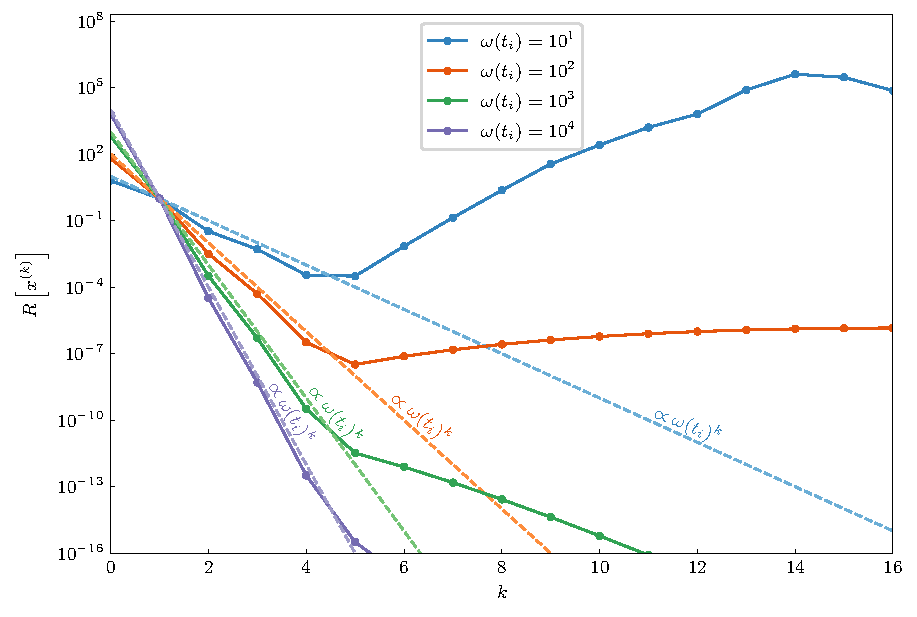
\includegraphics{plots/residual-k.pdf}
    \caption{\label{residual-reduction} Bla }
\end{figure}

\begin{figure}
    \centering
    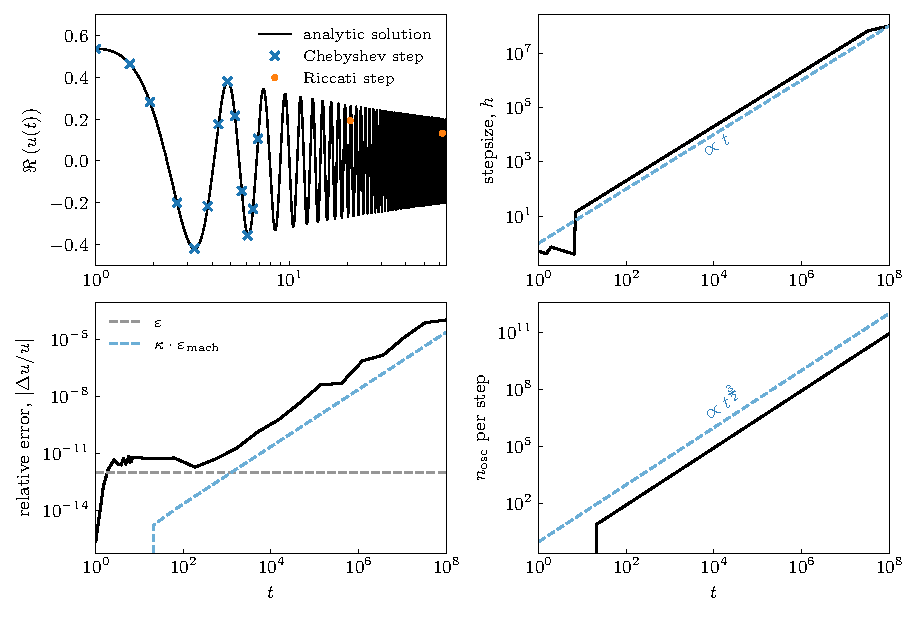
\includegraphics{plots/airy-numsol.pdf}
    \caption{\label{airy-results} Bla }
\end{figure}

\begin{figure}
    \centering
    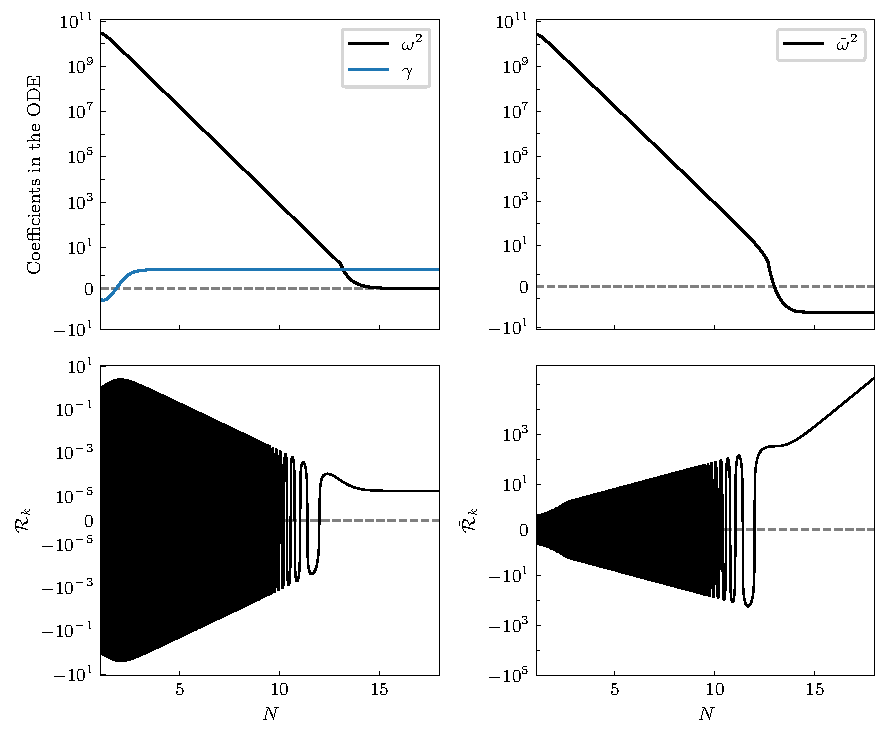
\includegraphics{plots/cosmology.pdf}
    \caption{\label{cosmology-example} Bla }
\end{figure}




% BBBBBBBBBBBBBBBBBBBBBBBBBBBBBBBBBBBBBBBBBBBBBBBBBBBBBBBBBBBBBBBBBBBBBBBBBBBB
\bibliographystyle{abbrv}
\bibliography{refs}
\end{document}

